\documentclass[16pt]{article}
\usepackage[english]{babel}
\usepackage{longtable}
\usepackage[top=1in, bottom=0.25in, left=1.25in, right=1.25in,includefoot,heightrounded]{geometry}
\usepackage{indentfirst}
\usepackage[utf8]{inputenc}
\usepackage{amsmath,amssymb}
\usepackage{graphicx,tikz}
\usepackage{hyperref}
\usepackage[colorinlistoftodos]{todonotes}
\usepackage[document]{ragged2e}
\usepackage{fancyhdr}
\usepackage{enumerate}
\usepackage{listings}
\usepackage{color}
\usepackage{flowchart}
\usepackage{hyperref}
\usepackage{graphicx}
\usetikzlibrary{arrows}


\usetikzlibrary{shapes.geometric, arrows}
\tikzstyle{startstop} = [rectangle, rounded corners, minimum width=3cm, minimum height=1cm,text centered, draw=black, fill=red!30]
\tikzstyle{decision} = [diamond, minimum width=4cm, minimum height=0.5cm, text centered, draw=black, fill=green!30]
\tikzstyle{process} = [rectangle, minimum width=3cm, minimum height=1cm, text centered, draw=black, fill=orange!30]
\tikzstyle{arrow} = [thick,->,>=stealth]
\tikzstyle{io} = [trapezium, trapezium left angle=70, trapezium right angle=110, minimum width=2cm, text width=4cm, minimum height=1cm, text centered, draw=black, fill=blue!30]

\pagestyle{fancy}
\fancyhf{}
\lhead{Myles Deslippe}
\rhead{Comp 3670 | Computer Networks}
\cfoot{\thepage}

\definecolor{MyDarkGreen}{rgb}{0.0,0.4,0.0}
\lstset{inputencoding=ansinew}
\lstset{breaklines=true} 

\begin{document}

    \section*{\centering{Transport Services and Protocols}}

    \subsection*{Transport Services and Protocols}
    \begin{itemize}
        \item The \textbf{transport layer} is responsible for providing \textbf{logical communication} between \textbf{application procceses} running on \textbf{different hosts}.
        \item There are two actions the transport layer needs to achieve:
        \begin{enumerate}
            \item \textbf{Send action}: The transport layer needs to \textbf{divide application messages into segments}, and pass them to the \textbf{network layer}.
            \item \textbf{Recieve action}: The transport layer needs to \textbf{reassemble segments} from the \textbf{network layer} into \textbf{messages}, and pass them to the \textbf{application layer}.
        \end{enumerate}
        \item There are \textbf{two transport protocols} available: the \textbf{User Datagram Protocol (UDP)}, and the \textbf{Transmission Control Protocol (TCP)}.
    \end{itemize}

    \subsection*{The Application Layer, The Transport Layer, and The Network Layer}
    \begin{itemize}
        \item The \textbf{application layer} is the \textbf{process} that is running on the \textbf{network host}.
        \item The \textbf{transport layer} is responsible for the \textbf{logical communcation} between \textbf{processes}.
        \item The \textbf{network layer} is responseible for the \textbf{logical communication} between \textbf{network hosts}.
        \item When a \textbf{message is sent} from an application over the network, it follow the following order: application layer $\rightarrow$ transport layer $\rightarrow$ network layer.
        \item When a \textbf{message is received} from the network, and sent to an application, it follows the following order: network layer $\rightarrow$ transport layer $\rightarrow$ application layer.
    \end{itemize}

    \subsection*{Transport Layer Actions}
    \begin{itemize}
        \item When a message is \textbf{sent from an application}, the \textbf{transport layer} does the following:
        \begin{enumerate}
            \item Recieves the application-layer message.
            \item Determines segment header field values.
            \item Creates the segment.
            \item Passes the segment to the internet protocol.
        \end{enumerate}
        \item When a message is \textbf{recieved from the network}, the \textbf{transport layer} does the following:
        \begin{enumerate}
            \item Recieves the segment from the internet protocol.
            \item Checks the header values.
            \item Extracts the application-layer message.
            \item Demultiplexes message up to the application via a socket.
        \end{enumerate}
    \end{itemize}

    \subsection*{User Datagram Protocol and Transmission Control Protocol}
    \begin{itemize}
        \item The \textbf{User Datagram Protocol (UDP)} is an \textbf{unreliable}, \textbf{unordered} delivery protocol. This protocol has \textbf{minimal overhead} but is \textbf{not reliable}.
        \item The \textbf{Transmission Control Protocol (TCP)} is a \textbf{reliable}, \textbf{in-order delivery} protocol that supports \textbf{congestion control}, \textbf{flow control}, and \textbf{connection setup}. This protocol has \textbf{significant overhead}, but is \textbf{very reliable}.
        \item Both \textbf{UDP} and \textbf{TCP} do not provide \textbf{delay guarantees} and \textbf{bandwith guarantees}.
    \end{itemize}

    \section*{\centering{Multiplexing}}
    
    \subsection*{Multiplexing}
    \begin{itemize}
        \item \textbf{Multiplexing} is a method used by \textbf{networks} to \textbf{consolidate multiple signals} into a \textbf{single composit signal} that is then \textbf{transported over a common medium}. 
        \item When \textbf{sending data}, \textbf{multiplexing} is used to \textbf{transmit segments} from \textbf{several sockets} via \textbf{transport headers}.
        \item When \textbf{recieving data}, the \textbf{header info} is used to \textbf{demultiplex} the data, sending it to the \textbf{correct socket}.
        \item \textbf{Demultiplexing} works by receiving \textbf{IP datagrams} containing a \textbf{source and destination IP address and port as headers}. Each datagram contains a \textbf{single segment}.
        \begin{itemize}
            \item The IP addresses and port numbers are used to route the segment to the correct socket.
            \item This is why you must specify a port (and sometimes an address) number when creating a socket.
        \end{itemize} 
    \end{itemize}

    \subsection*{Connectionless Multiplexing}
    \begin{itemize}
        \item When creating a \textbf{server socket} you must specify a \textbf{port}, that the \textbf{socket will be bound to}.
        \item When creating a \textbf{datagram (UDP)} you must specify the \textbf{destination host and port}.
        \item When a \textbf{host} receives a \textbf{datagram} with the \textbf{port destination} that matches the \textbf{port the server socket is bound to}, it will \textbf{route the datagram} to \textbf{said socket}.
        \begin{itemize}
            \item The host address does not matter when a datagram is recieved by a host, it will simply attempt to route it to the destination port. This means that several hosts can send datagrams to the same port, and they will all be available at the same socket.
        \end{itemize}  
    \end{itemize}

    \subsection*{Connection-Oriented Multiplexing}
    \begin{itemize}
        \item When creating a \textbf{connection oriented socket (TCP)}, you create a \textbf{4-tuple} containing the \textbf{source address, source port, destination address, and destination port}.
        \item The \textbf{4-tuple} is used to \textbf{route inbound packets} to the \textbf{correct socket}.
        \item \textbf{Servers} may support \textbf{several simultaneous TCP sockets}, typically one for \textbf{each client}. Each socket will have a \textbf{unique 4-tuple}.
    \end{itemize}

    \subsection*{Summary}
    \begin{itemize}
        \item Multiplexing and demultiplexing are based on segman, datagram header values.
        \item UDP uses the port for demultiplexing.
        \item TCP uses the 4-tuple for demultiplexing.
        \item Multiplexing happens at all layers.
    \end{itemize}
    
    \section*{\centering{User Datagram Protocol}}

    \subsection*{User Datagram Protocol}
    \begin{itemize}
        \item The \textbf{User Datagram Protocol (UDP)} is a \textbf{connectionless (no handshake)} \textbf{communication protocol} that uses the \textbf{internet protcol}.
        \item \textbf{UDP} has \textbf{minimal overhead}, at the cost of having \textbf{no connection state, no congestion control, and no packet delivery verification}.
        \item \textbf{UDP} is used for \textbf{loss-tolerant, rate sensitive} applications.
        \item It is possible to have \textbf{reliable UDP communication} by implementing it at the \textbf{application layer}.
        \item[] \begin{center}
                    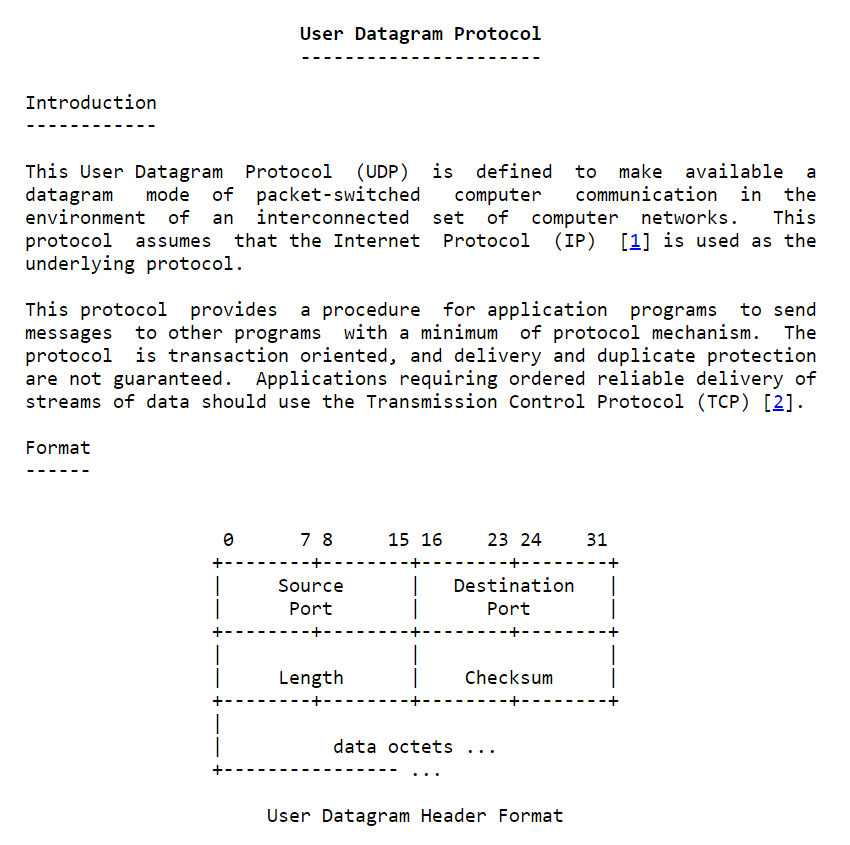
\includegraphics[height=300px]{images/UDP.PNG}
                \end{center}
        \item \textbf{UDP datagrams} have the following headers:
        \begin{enumerate}
            \item \textbf{Destination port} | The port the datagram is being sent to.
            \item \textbf{Length} | The length in octets of the datagram.
            \item \textbf{Checksum} | The checksum is used to ensure the packet received was not corrupted during transmission.
            \item \textbf{Pseudo} | A header containing the source address, destination address, the protocol, and the UDP length. This information is used to give protection against misrouted datagrams.
        \end{enumerate} 
        \item The \textbf{checksum} is computed by taking the \textbf{one's complement sum} of the \textbf{entire content} of the \textbf{datagram}, treating the bits of the datagram as a \textbf{series of 16-bit integers}.
        \begin{itemize}
            \item The checksum is not perfect, several different datagrams can result in the same checksum.
        \end{itemize}
    \end{itemize}

    \section*{\centering{Reliable Data Transfer}}

    \subsection*{Reliable Data Transfer Overview}
    \begin{itemize}
        \item The \textbf{complexity} of the \textbf{reliable data transfer protocol} will strongly \textbf{depend} on the \textbf{characteristics} of the \textbf{unreliable channel} (drop packes, corruption, data reordering, etc).
        \item The \textbf{sender} and \textbf{receiver} \textbf{do not know the state of each other}, unless it is \textbf{communicated}.
    \end{itemize}

    \subsection*{RDT 1.0 | Reliable Transfer over a Reliable Channel}
    \begin{itemize}
        \item In this case, the \textbf{underlying channel} is perfectly \textbf{reliable}; there are \textbf{no bit errors}, and \textbf{no loss of packets}.
        \item This is the most primitive form of reliable data transfer; the \textbf{sender sends the data}, and the \textbf{receiver reads the data}.
        \item[] \includegraphics*[width=\textwidth - 25pt]{images/RDT-1.0.PNG}
    \end{itemize}
    
    \subsection*{RDT 2.0 | Channel with Bit Errors}
    \begin{itemize}
        \item In this case, the \textbf{underlying channel} may \textbf{flip bits in packets randomly}. To determine if this happend we can use a \textbf{checksum}.
        \item To \textbf{recover from errors}, we can have the \textbf{receiver send a respone}.
        \begin{itemize}
            \item The \textbf{acknowledgement (ACK) response} indicates that the \textbf{packet was successfully transmitted}.
            \item The \textbf{negative acknowledgement (NAK) response} indicates that the \textbf{packet was not successfully transmitted}.
            \item If the \textbf{sender} recieves a \textbf{NAK response}, they must \textbf{retransmit the packet}.
        \end{itemize} 
        \item The \textbf{sender} must \textbf{stop and wait} for a resonse, before sending the next packet.
        \item[] \includegraphics*[width=250px]{images/RDT-2.0.PNG} \includegraphics*[width=100px]{images/RDT-2.0-1.PNG}
        \item \textbf{RDT 2.0 has a fatal flaw}, if the \textbf{ACK} or \textbf{NAK} gets \textbf{corrupted}, the \textbf{sender} won't know if the \textbf{receiver} received the packet.
        \begin{itemize}
            \item You can't retransmit the packet, it could result in a possible duplicate.
        \end{itemize} 
    \end{itemize}

    \subsection*{RDT 2.1 | Handling Corrupted ACKs and NAKs}
    \begin{itemize}
        \item In the case where the \textbf{receiver's response} gets \textbf{corrupted}, we can add a \textbf{sequence number to each packet}. This will allow the reciever to detect duplicate packets.
        \item[] \begin{center}
                    \includegraphics*[height=200px]{images/RDT-2.1.PNG}
                \end{center}
        \item[] \begin{center}
                   \includegraphics*[height=200px]{images/RDT-2.1-1.PNG}
                \end{center}
    \end{itemize}

    \subsection*{RDT 2.2 | A NAK-free Protocol}
    \begin{itemize}
        \item This protocol has the \textbf{same functionality as 2.1}, but it only uses \textbf{ACKs}.
        \item \textbf{Instead of NAK}, the \textbf{receiver} sends \textbf{ACK} for the \textbf{last packet recieved OK}.
        \begin{itemize}
            \item The receiver must explicitally include the sequence number of the packet being ACKed.
        \end{itemize}
        \item A \textbf{duplicated ACK} at the \textbf{sender} results in the \textbf{same action as NAK}; retransmit the current packet.
        \item[] \includegraphics*[width=\textwidth-25pt]{images/RDT-2.2.PNG}
    \end{itemize}

    \subsection*{RDT 3.0 | Channels with Bit Errors and Packet Loss}
    \begin{itemize}
        \item In this case the \textbf{underlying channel} can \textbf{lose packets, and corrupt packets}.
        \item The checksum, sequence of numbers, ACKs, and restransmission will help, but will not be enough.
        \item In this protocol, the \textbf{sender waits a "reasonable" anout of time} for an \textbf{ACK}, if \textbf{ACK is not recieved} within a reasonable amount of time, the \textbf{sender} will \textbf{retransmit the packet}.
        \begin{itemize}
            \item If the packet ACK was just delayed and not lost, the sequence number will allow to reciever to discard the duplicate packet.
            \item When the reciever is sending the ACK, they must specify the packet number they are ACKing.
        \end{itemize}
        \item[] \begin{center}
                    \includegraphics*[width=300px]{images/RDT-3.0.PNG} 
                \end{center}
        \item[] \begin{center}
                    \includegraphics*[width=300px]{images/RDT-3.0-1.PNG} 
                \end{center}
        \item The \textbf{stop-and-wait} operation the \textbf{sender} has to undergo is \textbf{very slow}; It reduces the maximum transmission rate.
    \end{itemize}

    \subsection*{RDT 3.0 | Pipelined Protocol Operations}
    \begin{itemize}
        \item \textbf{Pipelining} is when the \textbf{sender} allows for \textbf{multiple in-flight} (yet to be acknowledged) \textbf{packets}.
        \begin{itemize}
            \item The range of the sequence numbers must be increased.
            \item Buffering is required and the sender's end and the reciever's end.
        \end{itemize}
        \item \textbf{Pipelining} allows for increased utilization.
    \end{itemize}

    \subsection*{RDT 3.0 | Pipelined Go-Back-N Protocol}
    \begin{itemize}
        \item In the \textbf{Go-Back-N protocol}, the \textbf{sender} sends a \textbf{"window"} of up to \textbf{N}, consecutively transmitted (unacknowldeg) \textbf{packes}.
        \item After the sender recieves a \textbf{cumulative ACK} (acknowledgement of all packets up to n), the \textbf{sender} moves the \textbf{window forward to begin at n+1}.
        \item If a timeout occurs, simply retransmit the window.
        \item In the \textbf{Go-Back-N protocol}, the \textbf{receiver} sends an \textbf{ACK} for the \textbf{correctly-received packets} so far, with the highest \textbf{in-order} sequence numbers (This may generate duplicate ACKs).
        \item If the \textbf{receiver} receives \textbf{out-of-order packets}, they can either reorder them, or discard and re-ACK (it depends on the implementation).
    \end{itemize}

    \subsection*{RDT 3.0 | Pipelined Selective Repeat Protocol}
    \begin{itemize}
        \item In the \textbf{Selective Repeat protocol}, the \textbf{receiver individually acknowledges} all \textbf{correctly received pacakets}.
        \begin{itemize}
            \item The receiver buffers the packets, as needed, for an eventual in-order delivery to the uppter layer.
        \end{itemize}
        \item The \textbf{sender retransmits unACKed packets}.
        \begin{itemize}
            \item The sender must maintain a timer for each unACKed packet.
        \end{itemize}
        \item[] \includegraphics*[width=\textwidth - 25pt]{images/Selective-Repeat-Protocol.PNG}
    \end{itemize}

    \subsection*{Principals of Congestion Control}
    \begin{itemize}
        \item Informally, \textbf{congestion} occurs when \textbf{too may sources are sending data too fast} for a \textbf{network to handle}.
        \begin{itemize}
            \item Indicators that congestion is occuring are \textbf{long delays, and packet loss}.
        \end{itemize}
        \item One the indicators of congestion occur, the sender should act accordingly.
        \item There is also \textbf{network-assisted congestion control}; \textbf{routers} provide \textbf{direct feedback} to the \textbf{sending} and \textbf{receiving} hosts (may indicate congestion level as-well).
    \end{itemize}

    \section*{\centering{Connection-Oriented Transportation: TCP}}

    \subsection*{Transmission Control Protocol (TCP) Overview}
    \begin{itemize}
        \item TCP is is/does the following:
        \begin{enumerate}
            \item \textbf{Point-To-Point}: There is one sender, and one receiver.
            \item \textbf{Reliable, in-order byte stream}: There are no "message boundaries".
            \item \textbf{Full Duplex}: There is bi-directional data flow in a single connection.
            \item \textbf{Pipelined}: TCP congestion and flow-control can set the window size.
            \item \textbf{Connection-Oriented}: Handshaking is used to initalize the sender and receiver state before the data exchange begins.
            \item \textbf{Flow Controlled}: The sender will not overwhelm the receiver.
            \item \textbf{Supports cumulative ACKs}.
        \end{enumerate}
        \item The \textbf{TCP specification does not specify} how to handle \textbf{out-of-order packets}; it is up to the specific implementation. 
        \item The \textbf{TCP timeout period} must be carefully set. If it is \textbf{too short}, premature timeout occurs. If it is \textbf{too long}, there is a slow reaction to segment loss.
        \item To estimate the \textbf{route-trip time (RTT)} you do the following:
        \begin{enumerate}
            \item Measure the time starting when a single segmant transmisstion is sent, and stopping when you receive an ACK receipt. Set $EstimatedRTT$ equal to this time length.
            \item Repeat the process as your transmit more segments, updating the $EstimatedRTT$ with the following formula: $EstimatedRTT=(1-\alpha)\times{EstimatedRTT}+\alpha\times{SampleRTT}$ (A typical $\alpha$ value is 0.125).
        \end{enumerate}
        \begin{itemize}
            \item When actually setting the timeout period, you should add a \textbf{saftey margin}. 
        \end{itemize}
        \item \textbf{TCP Fast Re-Transmit}: When the \textbf{sender} receives \textbf{three ACKs} for \textbf{the same data}, the \textbf{sender} should \textbf{re-transmit all unACKed segments}.
    \end{itemize}

    \subsection*{TCP Segment Structure}
    \begin{itemize}
        \item[] \includegraphics*[width=\textwidth - 25pt]{images/TCP.PNG}
        \item \textbf{TCP segments} are \textbf{composed of 10 sections}:
        \begin{enumerate}
            \item \textbf{Source Port}: The port the segment is coming from.
            \item \textbf{Destination Port}: The port the segment is going to.
            \item \textbf{Sequence Number}: The number of bytes in the bytestream.
            \item \textbf{Acknowledgements}: Sequence number of the next byte expected from the other side, and cumulative ACKs.
            \item \textbf{Length and Flags}: The length of the TCP header, and other flags.
            \item \textbf{Receive Window}: The number of bytes the receiver is willing to accept (flow control).
            \item \textbf{Checksum}: A checksum to verify the segment was received correctly.
            \item \textbf{Url Data Pointer}: Indicates how many bytes from the first are urgent.
            \item \textbf{TCP Options}: Additional options (variable length).
            \item \textbf{Applicaton Data}: The payload (variable length).
        \end{enumerate}
    \end{itemize}

    \subsection*{TCP Connection Creation}
    \begin{itemize}
        \item \textbf{Before data} is \textbf{exchanged}, the \textbf{sender} and the \textbf{receiver} perform a \textbf{handshake}.
        \item This let's both sides know that \textbf{the other side agrees to establish a connection}, and that they \textbf{agree on connection parameters}.
        \item \textbf{TCP} uses a \textbf{3-way handshake} to establish a connection.
        \item[] \includegraphics*[width=\textwidth - 25pt]{images/TCPHandShake.PNG}
    \end{itemize}

    \subsection*{TCP Flow Control}
    \begin{itemize}
        \item \textbf{TCP flow control} is achieved by the \textbf{receiver} setting the \textbf{window section of the TCP segment} specifying \textbf{how many segments it is able to receive}.
        \item This will prevent the receiver from being overwhelmed.
    \end{itemize}

    \subsection*{TCP Connection Termination}
    \begin{itemize}
        \item To \textbf{terminate a TCP connection}, the \textbf{client} and the \textbf{server} both \textbf{close their side of the connection}; by sending a \textbf{TCP segment} with the \textbf{FIN} bit set to \textbf{1}.
        \item They respond to the \textbf{FIN} with \textbf{ACK}; the ACK response can be combined with FIN.
        \item Simultaneous FIN exchanges can be handled.
    \end{itemize}

    \subsection*{TCP Congestion Control: AIMD}
    \begin{itemize}
        \item \textbf{AIMD} stands for \textbf{Additive Increase, Multiplicative Decrease}.
        \item The \textbf{sender} can \textbf{increase the sending rate} until \textbf{congestion occurs}, then decrease.
        \begin{itemize}
            \item When increasing the transmission rate, you increase the sending rate by 1 maximum segment size every RTT until loss is detected.
            \item When decreasing the transmission rate, you cut the rate in half at each loss event.
        \end{itemize}
        \item \textbf{AIMD} has been shown to \textbf{optomize congested flow rates network-wide}, and is stable.
        \item When a \textbf{connection is first established}, the segments should start off being sent \textbf{really slow, and increase exponentially until lose occurs}. After \textbf{loss occurs}, follow the \textbf{AIMD} principals.
    \end{itemize}

\end{document}